% Template for ICASSP-2013 paper; to be used with:
%          spconf.sty  - ICASSP/ICIP LaTeX style file, and
%          IEEEbib.bst - IEEE bibliography style file.
% --------------------------------------------------------------------------
\documentclass{article}
\usepackage{spconf,amsmath,graphicx}
\usepackage{empheq}
\usepackage{tikz}
\usetikzlibrary{shapes,snakes}
\usetikzlibrary{calc,chains,positioning}
\usepackage{cases}
\usepackage{phaistos}
\DeclareMathOperator{\diag}{diag}
% Example definitions.
% --------------------
\def\x{{\mathbf x}}
\def\L{{\cal L}}

% Title.
% ------
\title{A Perceptually Constrained Channel Shortening Technique
\\ for Speech Dereverberation}
%
% Single address.
% ---------------
\name{Ina Kodrasi\textsuperscript{1}, Stefan Goetze\textsuperscript{2},  Simon Doclo\textsuperscript{1,2}~\thanks{This research was partly funded by the German-Israeli Foundation for Scientific Research and Development~(GIF).}}
\address{
%email of first author
%affiliation and address of first author
$^1$University of Oldenburg, Department of Medical Physics and Acoustics, Oldenburg, Germany\\
%affiliations of remaining authors
$^2$Fraunhofer IDMT, Project Group Hearing, Speech and Audio Technology, Oldenburg, Germany\\
{\tt ina.kodrasi@uni-oldenburg.de}
}


\begin{document}
\ninept
%
\maketitle
%
\begin{abstract}
The objective of acoustic multichannel equalization is to design a reshaping filter that reduces reverberation, improves the perceptual speech quality, and is robust to errors in the estimated room impulse responses~(RIRs).
Although the channel shortening~(CS) technique has been shown to be effective in achieving dereverberation, it may fail to preserve the natural shape of an RIR leading to speech quality degradation.
Furthermore, CS yields multiple reshaping filters that satisfy its optimization criterion but result in a different perceptual speech quality.

In this paper, we propose a robust perceptually constrained channel shortening technique~(PeCCS) that resolves the selection ambiguity of CS and leads to joint dereverberation and speech quality preservation.
Simulation results for erroneously estimated RIRs show that PeCCS preserves the perceptual speech quality and results in a higher reverberant tail suppression than other state-of-the-art techniques, such as CS and the regularized partial multichannel equalization technique based on the multiple-input/output inverse theorem~(P-MINT).

\end{abstract}
%
\begin{keywords}
acoustic multichannel equalization, channel shortening, robustness, speech dereverberation
\end{keywords}
%
\section{Introduction}
\label{sec:intro}
Acoustic multichannel equalization techniques aim at achieving speech dereverberation by reshaping the estimated room impulse responses~(RIRs) between the source and the microphone array.
Although in theory perfect dereverberation can be obtained when multiple microphones are available~\cite{Miyoshi_ITASS_1988,Hacihabibouglu_ITASLP_2012}, such an approach poses the practical challenge of achieving robustness to errors in the estimated RIRs~\cite{Hikichi_EURASIP_2007, Zhang_IWAENC_2010, Kodrasi_IWAENC_2012}.
Since the estimated RIRs typically differ from the true RIRs~\cite{Hasan_EUSIPCO_2006}, acoustic multichannel equalization techniques may fail to achieve dereverberation and may even lead to distortions in the output speech signal~\cite{Radlovic_ITSA_2000}.
In order to address this robustness issue, techniques such as regularized partial multichannel equalization based on the multiple-input/output inverse theorem~(P-MINT)~\cite{Kodrasi_IWAENC_2012} and channel shortening~(CS)~\cite{Zhang_IWAENC_2010,Kallinger_ICASSP_2006} have been proposed.

The regularized P-MINT technique aims at simultaneously suppressing the reverberant tail and controlling the perceptual speech quality of the output signal.
Experimental investigations in~\cite{Kodrasi_IWAENC_2012} have shown that regularized P-MINT outperforms state-of-the-art techniques such as CS in terms of perceptual speech quality.
However, the performance in terms of reverberant tail suppression is generally lower than CS.

The objective of CS is to design a reshaping filter which minimizes the reverberant energy while maximizing the energy of the direct path and early reflections.
Such an energy-based optimization technique typically achieves a high level of reverberant tail suppression, but may fail to preserve the general shape of a natural RIR, hence leading to a degraded speech quality~\cite{Kodrasi_IWAENC_2012}.
Furthermore, CS yields multiple reshaping filters which all satisfy its optimization criterion.
However, these reshaping filters result in a different perceptual speech quality~\cite{Zhang_IWAENC_2010}, raising the question of how to obtain a perceptually advantageous solution in practice.

In this paper, a method for resolving the selection ambiguity of a perceptually advantageous solution in CS is proposed.
The reshaping filter is designed as a linear combination of the multiple CS reshaping filters that leads to a reshaped overall response which is similar to the first part of one of the estimated RIRs. 
As a result, a robust perceptually constrained channel shortening technique~(PeCCS) is established, which jointly achieves reverberant tail suppression as well as perceptual speech quality preservation.

\section{Acoustic Multichannel Equalization}
\label{sec: ame}
\subsection{Configuration and notation}
Consider the $M$-channel acoustic system depicted in Fig.~\ref{fig: acsys}.
The $m$-th microphone signal $x_m(n)$ at time index $n$ is given by
\begin{equation}
  x_m(n) = s(n) \ast h_m(n), \; \; \; \;  m = 1, \ldots, \; M,
\end{equation}
where $\ast$ denotes convolution, $s(n)$ is the clean speech signal, and $h_m(n)$ denotes the RIR between the source and the $m$-th microphone.
\begin{figure}[b]
  \centering
  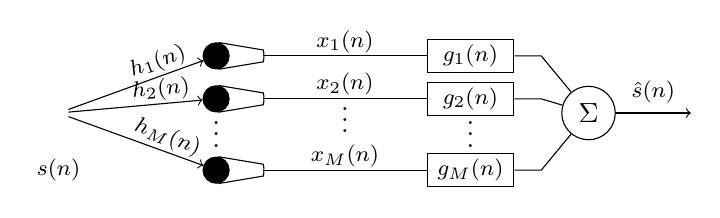
\begin{tikzpicture}
    % Adjustments
    \def\micd{.1cm}                % mic diameter
    \def\micl{.6cm}                % mic length
    \def\micw{.15cm}                % mic width
    \def\micbend{10}               % mic bottom bend
    \def\micdistance{.2cm}         % distance between microphones
    \def\filterdistance{2.5cm}     % distance between microphone and filter
    \def\filteroutline{.9cm}       % length of line which gets out of filter
    \def\sumdistance{1.5cm}        % distance of sum node to the filter
    \def\sumoutline{1cm}           % length of line which gets out of sum
    \def\headdistance{2cm}         % distance between microphone and head

    % Styles
    \tikzset{%
      mic head/.style={fill=black,draw=black,circle,minimum size=\micd},
      filter/.style={draw,minimum width=1.1cm,inner sep=2pt},
      sum/.style={draw,circle},
      xlabel/.style={inner sep=1pt,above,midway},
      sumlabel/.style={xlabel},
      hlabel/.style={xlabel,sloped,pos=.7},
      head/.style={font=\Large}
    }

    % Draw Microphones
    \begin{scope}[start chain=going below,every node/.style={on chain},node distance=\micdistance]
      \node[mic head] (mic1) {};
      \node[mic head] (mic2) {};
      \node[mic head,yshift=-1.8*\micdistance] (mic3) {};
    \end{scope}
    \node[yshift=3pt] at ($(mic2)!.5!(mic3)$) {$\vdots$};

    \foreach \m in {1,2,3} {%
      \coordinate (m1) at ($(mic\m)+(\micl,\micw/2)$);
      \coordinate (m2) at ($(mic\m)+(\micl,-\micw/2)$);
      \draw (tangent cs:node=mic\m,point={(m1)},solution=1) -- (m1) to[bend left=\micbend] (m2) -- (tangent cs:node=mic\m,point={(m2)},solution=2);
    }

    % Draw Filter
    \foreach \m/\i in {1/1,2/2,3/M} {%
      \node[filter,right=\filterdistance of mic\m] (filter\m) {\footnotesize $g_{\i}(n)$};
      \draw ($(mic\m)+(\micl,0)$) to node[xlabel] (x\m) {\footnotesize $x_{\i}(n)$} (filter\m);
    }
    \node[yshift=3pt] at ($(filter2)!.5!(filter3)$) {$\vdots$};
    \node[yshift=3pt] at ($(x2)!.5!(x3)$) {$\vdots$};
    % Sum Node
    \node[sum] (sum) at ($(filter1)!.5!(filter3)+(\sumdistance,0)$) {$\Sigma$};
    \draw[->] (sum) -- node[above] {\footnotesize $\hat{s}(n)$} ++(1.3,0);
    % Connect filter with sum
    \foreach \m in {1,2,3} {%
      \draw (filter\m) -- ++(\filteroutline,0) -- (sum);
    }

    % Head
    \node[head] (head) at ($(mic1)!.5!(mic3)-(\headdistance,0)$) {\PHtattooedHead};
    \node[fill=white,minimum width=4.8pt,minimum height=5.7pt,inner sep=0pt] at ($(head.center)+(2.3pt,-2.5pt)$) {};
    \node at ($(head.center)+(0.0pt,-20.5pt)$) {\footnotesize $s(n)$};
    % Connect head with mics
    \foreach \m/\i in {1/1,2/2,3/M} {%
      \draw[->] (head) -- node[hlabel] {\footnotesize $h_{\i}(n)$} (mic\m);
    }
  \end{tikzpicture}
  \caption{Multichannel equalization system}
  \label{fig: acsys}
\end{figure}
The RIR can be described in vector notation as 
\begin{equation}
\mathbf{h}_m = [h_m(0) \; h_m(1) \; \ldots \; h_m(L_h-1)]^T,
\end{equation} 
with $L_h$ being the RIR length and $[\cdot]^T$ denoting the transpose operation.
Applying reshaping filters $\mathbf{g}_m$ of length $L_g$, i.e. 
\begin{equation}
\mathbf{g}_m = [g_m(0) \; g_m(1) \; \ldots \; g_m(L_g-1)]^T,
\end{equation}
the output signal $\hat{s}(n)$ is given by the sum of the filtered microphone signals, i.e.
\begin{equation}
  \hat{s}(n)  = \sum_{m=1}^M x_m(n) \ast g_m(n) =  s(n) \ast \underbrace{\sum_{m=1}^M h_m(n) \ast g_m(n)}_{c(n)},
\end{equation}
where $c(n)$ denotes the equalized impulse response~(EIR) of length $L_c = L_h+L_g-1$, which can be described in vector notation as $\mathbf{c} = [c(0) \; c(1) \; \ldots \; c(L_c-1)]^T$.
Using the stacked $ML_g$-dimensional reshaping filter $\mathbf{g}$, i.e.
\begin{equation}
  \mathbf{g} = [\mathbf{g}_1^T \; \mathbf{g}_2^T \; \ldots \; \mathbf{g}_M^T]^T,
\end{equation}
and the $L_c \times ML_g$-dimensional multichannel convolution matrix $\mathbf{H}$, i.e.
\begin{equation}
  \mathbf{H} = [\mathbf{H}_1 \; \mathbf{H}_2 \; \ldots \; \mathbf{H}_M],
\end{equation}
with $\mathbf{H}_m$ being the $L_c \times L_g$-dimensional convolution matrix of $\mathbf{h}_m$, i.e.
\begin{equation}
\hspace{-0.2cm}
\mathbf{H}_m =  \begin{bmatrix}
    h_m(0) & 0 &  \ldots & 0 \\
    h_m(1) & h_m(0) & \ddots & \vdots \\
    \vdots & h_m(1) & \ddots & 0 \\
    h_m(L_h-1) & \vdots & \ddots & h_m(0) \\
    0 & h_m(L_h-1) & \ddots & h_m(1) \\
    \vdots & \ddots & \ddots & \vdots \\
    0 & \ldots & 0 & h_m(L_h-1)
   \end{bmatrix},\hspace{-0.4cm}
 \end{equation}
the EIR can be expressed as
\begin{equation}
  \label{eq: trueeir}
  \boxed{\mathbf{c} = \mathbf{H} \mathbf{g}}
\end{equation}
The convolution matrix $\mathbf{H}$ is assumed to be a full row-rank matrix~\cite{Harikumar_ITSP_1998}, and the length of the reshaping filters is assumed to be $L_g \geq \lceil \frac{L_h-1}{M-1} \rceil$~\cite{Miyoshi_ITASS_1988}.
The reshaping filter $\mathbf{g}$ can then be constructed based on different design objectives for the EIR $\mathbf{c}$.

However, since the true RIRs are generally not available in practice, acoustic multichannel equalization techniques design $\mathbf{g}$ using the estimated multichannel convolution matrix $\hat{\mathbf{H}}$~(constructed from the estimated RIRs $\hat{\mathbf{h}}_m$).
Hence, the estimated EIR $\hat{\mathbf{c}} = \hat{\mathbf{H}}\mathbf{g}$ is typically optimized instead of the true EIR in~(\ref{eq: trueeir}).
Several techniques which aim at decreasing the sensitivity of the reshaping filter $\mathbf{g}$ to RIR estimation errors have been proposed, of which the regularized P-MINT and the CS techniques are briefly reviewed in the following.

\subsection{Regularized partial multichannel equalization based on the multiple-input/output inverse theorem~(P-MINT)}
The objective of the regularized P-MINT technique~\cite{Kodrasi_IWAENC_2012} is to suppress the reverberant tail of the EIR while also preserving the general shape of a natural RIR.
This is achieved by defining the desired EIR to be $\hat{\mathbf{h}}_p^{\rm d}$, which denotes the first part~(i.e. direct path and early reflections) of one of the estimated RIRs, i.e.
\begin{equation}
\hat{\mathbf{h}}_{p}^{\rm d} = [\underbrace{0\phantom{\rlap{$(L_d-1)$}} \ldots 0 }_{\tau} \underbrace{\hat{h}_p(0) \ldots \hat{h}_p(L_d-1)}_{L_d} 0 \ldots 0 ]^{T},
\end{equation}
with $\tau$ being a delay in number of samples, $L_d$ denoting the length of the direct path and early reflections in number of samples, and $p \in \{1, \; \ldots, \; M\}$.
In order to decrease the sensitivity of the reshaping filter to errors in the estimated RIRs, a regularization term needs to be incorporated, leading to the regularized P-MINT cost function
\begin{equation}
  \label{eq: rpmintcost}
  \boxed{J_{_{\rm P-MINT}}^{{\rm R}} = \|\hat{\mathbf{H}}\mathbf{g} - \hat{\mathbf{h}}_p^{\rm d}\|_2^2 + \delta \|\mathbf{g}\|_2^2}
\end{equation}
with $\delta$ being a regularization parameter.
The regularized P-MINT reshaping filter minimizing~(\ref{eq: rpmintcost}) can be computed as
\begin{equation}
  \label{eq: rpmintsol}
  \boxed{\mathbf{g}_{_{\rm P-MINT}}^{{\rm R}} = (\hat{\mathbf{H}}^T\hat{\mathbf{H}}+\delta \mathbf{I})^{-1} \hat{\mathbf{H}}^T \hat{\mathbf{h}}_p^{\rm d}}
\end{equation}
with $\mathbf{I}$ being the $ML_g \times ML_g$-dimensional identity matrix.
In~\cite{Kodrasi_IWAENC_2012} it has been experimentally validated that such a technique is preferable in terms of perceptual speech quality.
However, its performance in terms of reverberant tail suppression is typically lower than other state-of-the-art multichannel equalization techniques.
\subsection{Channel shortening~(CS)}
CS has been extensively investigated in the context of digital communication applications~\cite{Martin_ITSP_2005} and has recently been applied to acoustic system equalization~\cite{Zhang_IWAENC_2010,Kallinger_ICASSP_2006}.
The objective of CS is to maximize the energy in the first $L_d$ taps~(i.e. direct path and early reflections) of the EIR, while minimizing the energy in the remaining taps~(i.e. reverberant tail).
This objective can be expressed in terms of a generalized Rayleigh quotient maximization problem, i.e.
\begin{equation}
  \label{eq: cscost}
  \boxed{J_{_{\rm CS}} = \frac{\|\mathbf{W}_d \hat{\mathbf{H}}\mathbf{g} \|_2^2}{\|\mathbf{W}_u \hat{\mathbf{H}}\mathbf{g} \|_2^2} = \frac{\mathbf{g}^T\hat{\mathbf{B}}\mathbf{g}}{\mathbf{g}^T\hat{\mathbf{A}}\mathbf{g}}}
\end{equation}
where $\mathbf{W}_d$ and $\mathbf{W}_u$ are diagonal matrices representing the desired and undesired windows respectively, i.e.
\begin{align}
\label{eq: wincs}
\mathbf{W}_d & = {\diag} \{ [\underbrace{0 \; \ldots \; 0}_{\tau} \; \underbrace{1 \; \ldots \; 1}_{L_d}\; 0\; \ldots\; 0] \},  \\
\mathbf{W}_u & =  {\diag} \{ [\underbrace{1 \; \ldots \; 1}_{\tau} \; \underbrace{0 \; \ldots \; 0}_{L_d}\; 1\; \ldots\; 1] \},
\end{align}
and
\begin{align}
\hat{\mathbf{B}} & = \hat{\mathbf{H}}^{T} \mathbf{W}_d^T\mathbf{W}_d\hat{\mathbf{H}},  \\
\hat{\mathbf{A}} & = \hat{\mathbf{H}}^{T}\mathbf{W}_u^T\mathbf{W}_u \hat{\mathbf{H}}.
\end{align} 
Maximizing~(\ref{eq: cscost}) is equivalent to solving the generalized eigenvalue problem $\hat{\mathbf{B}}\mathbf{g} = \lambda \hat{\mathbf{A}}\mathbf{g}$, where the optimal reshaping filter $\mathbf{g}_{_{\rm CS}}$ is the generalized eigenvector corresponding to the largest generalized eigenvalue $\lambda_{\max}$, i.e.
\begin{equation}
  \label{eq: cssol}
  \boxed{\hat{\mathbf{B}}\mathbf{g}_{_{\rm CS}} = \lambda_{\max}\hat{\mathbf{A}}\mathbf{g}_{_{\rm CS}}}
\end{equation}
In~\cite{Zhang_IWAENC_2010} it has been shown that there exist $L_d$ linearly independent generalized eigenvectors satisfying~(\ref{eq: cssol}), which however yield a different perceptual speech quality.
Furthermore, also a selection criterion has been proposed in~\cite{Zhang_IWAENC_2010}, namely the generalized eigenvector leading to the minimum $l_2$-norm EIR.
However, this criterion is based on observations using informal listening tests for perfectly estimated RIRs.

In the following, we propose a method for deriving a perceptually advantageous solution in the presence of RIR estimation errors, which is a linear combination of all generalized eigenvectors satisfying~(\ref{eq: cssol}).
The experimental results in Section~\ref{sec: exp} validate the advantages of the proposed method.

\section{Perceptually Constrained \\ Channel Shortening~(PeCCS)}
Consider the $ML_g \times L_d$-dimensional matrix $\mathbf{G}_{_{\rm CS}}$ whose columns are the generalized eigenvectors $\mathbf{g}_{_{\rm CS}}^k$, $k= 1, \; \ldots, \; L_d$, satisfying~(\ref{eq: cssol}), i.e.
\begin{equation}
  \mathbf{G}_{_{\rm CS}} = [\mathbf{g}_{_{\rm CS}}^1 \; \mathbf{g}_{_{\rm CS}}^2 \; \ldots \; \mathbf{g}_{_{\rm CS}}^{L_d}].
\end{equation}
Then, any linear combination of these generalized eigenvectors, i.e.
\begin{equation}
  \label{eq: lc}
  \mathbf{g} = \mathbf{G}_{_{\rm CS}}\boldsymbol\alpha,
\end{equation}
with $\boldsymbol \alpha$ being an $L_d$-dimensional vector of scalar coefficients, also maximizes the generalized Rayleigh quotient in~(\ref{eq: cscost}).
In order to obtain a reshaping filter that also yields a high perceptual speech quality, we propose to compute the vector $\boldsymbol \alpha$ minimizing the cost function
\begin{equation}
  \label{eq: peccscost}
 \boxed{J_{_{\rm PeCCS}} =  \|\hat{\mathbf{H}}\mathbf{G}_{_{\rm CS}} \boldsymbol \alpha - \hat{\mathbf{h}}_p^{\rm d} \|_2^2 + \|\mathbf{G}_{_{\rm CS}}\boldsymbol \alpha \|_2^2}
\end{equation}
The first term in~(\ref{eq: peccscost}) aims to obtain a reshaping filter that preserves the first taps of one of the estimated RIRs whereas the second term controls the reshaping filter energy in order to decrease its sensitivity to errors in the estimated RIRs.
Clearly, the weight given to the minimization of the energy of the reshaping filter in~(\ref{eq: peccscost}) can be controlled by incorporating a regularization parameter as done in the regularized P-MINT technique~(cf.~(\ref{eq: rpmintcost})).
However, the analysis of such a regularized technique is beyond the scope of this paper.

By setting the derivative of~(\ref{eq: peccscost}) with respect to $\boldsymbol \alpha$ equal to $\mathbf{0}$, the vector $\boldsymbol \alpha_{_{\rm PeCCS}}$ minimizing $J_{_{\rm PeCCS}}$ can be computed as
\begin{empheq}[box=\fbox]{align}
   \boldsymbol \alpha_{_{\rm PeCCS}} & = [(\hat{\mathbf{H}}\mathbf{G}_{_{\rm CS}})^T(\hat{\mathbf{H}}\mathbf{G}_{_{\rm CS}}) + \mathbf{G}_{_{\rm CS}}^T\mathbf{G}_{_{\rm CS}}]^{-1} \nonumber  \\
  & \times (\hat{\mathbf{H}}\mathbf{G}_{_{\rm CS}})^T (\hat{\mathbf{h}}_p^{\rm d})
\end{empheq}
leading to the PeCCS reshaping filter
\begin{equation}
  \boxed{\mathbf{g}_{_{\rm PeCCS}} = \mathbf{G}_{_{\rm CS}}\boldsymbol \alpha_{_{\rm PeCCS}}}
\end{equation}
The proposed PeCCS technique is hence a two-step multichannel equalization technique, which exploits the CS multiple solutions that already achieve reverberant tail suppression in order to obtain a robust and perceptually advantageous reshaping filter.


\section{Experimental Results}
\label{sec: exp}
In this section, the proposed PeCCS technique is compared to the CS~\cite{Zhang_IWAENC_2010} and regularized P-MINT~\cite{Kodrasi_IWAENC_2012} techniques.
\subsection{Simulation parameters and performance measures}
We have considered an acoustic scenario with a single speech source and $M=2$ microphones in a room with reverberation time $T_{60} \approx 600$~ms. 
The RIRs have been measured using the swept-sine technique with $L_h = 4800$ at a sampling frequency $f_s = 8$~kHz.
In order to simulate estimation errors, the measured RIRs have been perturbed by adding scaled white noise as proposed in~\cite{Cho_ITSA_1999}, i.e.
\begin{equation}
  \hat{h}_m(n) = h_m(n)[1+e(n)],
\end{equation}
with $e(n)$ being an uncorrelated Gaussian noise sequence with zero mean and an appropriate variance, such that a normalized channel mismatch $E_m$, defined as
\begin{equation}
  E_m = 10 \log_{10} \frac{\|\mathbf{h}_m - \hat{\mathbf{h}}_m \|_2^2}{\| \mathbf{h}_m\|_2^2},
\end{equation}
is generated.
Although other normalized channel mismatch values have been investigated, due to space constraints only $E_m = -33$~dB is considered in this paper.
Furthermore, the simulation parameters are set to $L_g = 4799$, $\tau = 0$, $p = 1$, and several desired window lengths have been considered, i.e.
\begin{equation}
  L_s = L_d \frac{1000}{f_s} \in \{20~\hbox{ms}, \; 30~\hbox{ms}, \; 40~\hbox{ms}, \; 50~\hbox{ms} \}.
\end{equation}

The suppression of the reverberant tail is evaluated using the energy decay curve~(EDC) of the EIR defined as
\begin{equation}
 \hbox{EDC}(n)\! = \!10 \log_{10}\frac{1}{\|\mathbf{c}\|_2^2}\sum_{i=n}^{L_c-1}c^2(i), \; n = 0,  \ldots,  L_c-1,
\end{equation}
where $\mathbf{c} = \mathbf{H}\mathbf{g}$ and the reshaping filter $\mathbf{g}$ is designed using the estimated convolution matrix $\hat{\mathbf{H}}$ for all considered techniques.

A commonly used perceptually motivated objective criterion which indicates how much of the non-direct path energy will be perceived as coloration instead of reverberation is the clarity index $C_{L_s}$~\cite{Naylor_Derev_book}, defined as
\begin{equation}
  C_{L_s} = 10 \log_{10}  \frac{\sum_{n = 0}^{L_d-1} c^2(n)}{\sum_{n = L_d}^{L_c-1} c^2(n)}.
\end{equation}
Furthermore, it has been shown in~\cite{Goetze_AES_2010} that measures relying on auditory models exhibit the highest correlation with subjective listening tests when evaluating the quality of dereverberated speech.
Hence, to evaluate the perceptual speech quality we have used the objective speech quality measure PESQ~\cite{PESQ}, where the reference signal employed in PESQ is $s(n) \ast h_1^{\rm d}(n)$, i.e. the clean speech signal convolved with the first part of the true first RIR for each value of the desired window length $L_s$.

For the CS technique, the reshaping filter is selected as the generalized eigenvector leading to the minimum $l_2$-norm estimated EIR $\hat{\mathbf{c}}$ as proposed in~\cite{Zhang_IWAENC_2010}. Furthermore, for the regularized P-MINT technique the regularization parameter $\delta$ in~(\ref{eq: rpmintsol}) is determined as in~\cite{Kodrasi_IWAENC_2012}, i.e. a set of regularization parameters $\delta \in \{10^{-9}, \; 10^{-8}, \; \ldots, \; 10^{-1} \}$ is considered, and the optimal parameter is selected as the one leading to the highest PESQ score.
It should be noted that such a procedure is intrusive and inapplicable in practice, since knowledge of the true RIRs is required to compute the true EIR $\mathbf{c}$ and to compute the reference signal $s(n) \ast h_1^{\rm d}(n)$ for PESQ.

\subsection{Results}
Fig.~\ref{fig: edc} depicts the EDC of the true RIR $\mathbf{h}_1$ and the EDCs of the EIRs obtained using all considered techniques for the desired window length $L_s = 50$~ms.
As can be observed in this figure, the generalized CS eigenvector leading to the minimum $l_2$-norm estimated EIR yields an EDC that is only slightly lower than the EDC of $\mathbf{h}_1$.
On the other hand, the regularized P-MINT technique achieves a higher level of reverberant tail suppression and the artificial tail introduced after $0.5$~s is not audible.
However, the proposed PeCCS technique yields the highest level of reverberant tail suppression throughout the duration of the RIR, with its reverberant tail being significantly below the reverberant tail of $\mathbf{h}_1$.
\begin{figure}[t!]
\centering
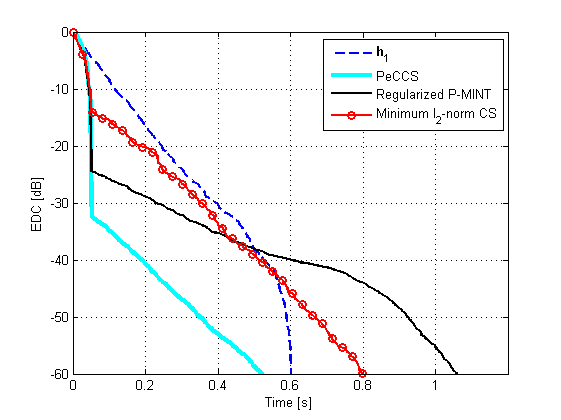
\includegraphics[scale=0.61]{Plots/EDC_5_-33}
\caption{EDC of the true RIR $\mathbf{h}_1$ and EDC of the EIR obtained using PeCCS, regularized P-MINT, and the generalized CS eigenvector leading to the minimum $l_2$-norm estimated EIR~($L_s = 50$~ms, $E_m = -33$~dB)}
\label{fig: edc}
\end{figure}
Fig.~\ref{fig: c50} shows the clarity index of $\mathbf{h}_1$ and the clarity index of the EIRs obtained using all considered techniques for different $L_s$.
The depicted $C_{L_s}$ values validate the previous conclusion based on the EDCs, i.e.~the proposed PeCCS technique yields the highest performance, followed by the regularized P-MINT technique.
The generalized eigenvector leading to the minimum $l_2$-norm estimated EIR yields the lowest clarity index for all considered desired window lengths $L_s$.

\begin{figure}[b!]
\centering
\includegraphics[scale=0.61]{Plots/Cxxn_simpar_5_simerror_-33}
\caption{Clarity index of the true RIR $\mathbf{h}_1$ and clarity index of the EIR obtained using PeCCS, regularized P-MINT, and the generalized CS eigenvector leading to the minimum $l_2$-norm estimated EIR~($E_m = -33$~dB)}
\label{fig: c50}
\end{figure}


Finally, we have evaluated the perceptual speech quality using PESQ for the different considered desired window lengths $L_s$.
The PESQ score of the first microphone signal $x_1(n)$ is also computed in order to determine the effectiveness of applying the considered dereverberation techniques.
The results are presented in Fig.~\ref{fig: pesq}, where it can be seen that the generalized CS eigenvector leading to the minimum $l_2$-norm estimated EIR yields the lowest perceptual speech quality for all considered $L_s$.
Furthermore, the proposed PeCCS technique yields a higher performance than the regularized P-MINT technique for $L_s = 20$~ms, $L_s = 30$~ms, and $L_s = 40$~ms, whereas a similar performance as the regularized P-MINT technique is obtained for $L_s = 50$~ms.


\begin{figure}[t!]
\centering
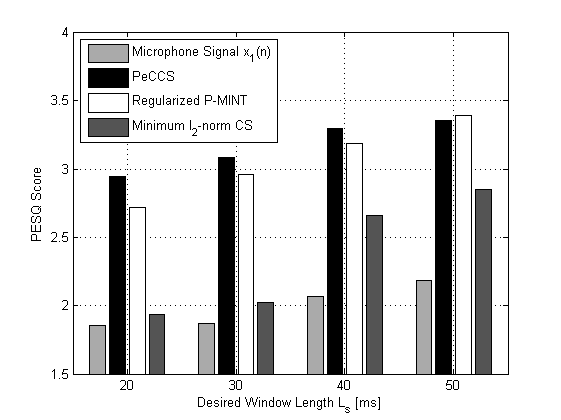
\includegraphics[scale=0.61]{Plots/PESQ_5_-33}
\caption{PESQ score of the first microphone signal $x_1(n)$ and PESQ score of the system's output $\hat{s}(n)$ obtained using PeCCS, regularized P-MINT, and the generalized CS eigenvector leading to the minimum $l_2$-norm estimated EIR~($E_m=-33$~dB)}
\label{fig: pesq}
\end{figure}


In conclusion, the presented simulation results demonstrate that applying the proposed PeCCS technique leads to a significantly higher level of reverberant tail suppression as well as speech quality preservation.

\section{Related Work}
To the best of our knowledge, the presented PeCCS technique is the first technique that considers the selection ambiguity of a perceptually advantageous solution in CS~\cite{Zhang_IWAENC_2010,Kallinger_ICASSP_2006} in the presence of RIR estimation errors.
In contrast to the selection criterion proposed in~\cite{Zhang_IWAENC_2010}, PeCCS takes into account RIR estimation errors and uses a novel optimization criterion which leads to a linear combination of the multiple CS solutions instead of a single generalized eigenvector.
Furthermore, unlike the regularized P-MINT technique proposed in~\cite{Kodrasi_IWAENC_2012}, PeCCS is a two-step multichannel equalization technique which exploits reshaping filters that already achieve reverberant tail suppression in order to derive a perceptually advantageous linear combination.

\section{Conclusion}
In this paper, we have presented a robust perceptually constrained acoustic multichannel equalization technique for speech dereverberation based on CS~(PeCCS).
Experimental results have shown that PeCCS achieves a significantly higher level of reverberant tail suppression than other state-of-the-art techniques such as CS and regularized P-MINT, while preserving the perceptual speech quality.

\pagebreak
\bibliographystyle{IEEEbib}
\bibliography{strings,refs}

\end{document}
